\documentclass[logo,reportComp]{thesis}
\usepackage[cpp,linenum]{mypackage}

\title{计算机图形学}
\subtitle{作业五:多边形网格}
\school{数据科学与计算机学院}
\author{陈鸿峥}
\classname{17大数据与人工智能}
\stunum{17341015}
\headercontext{计算机图形学作业}

\begin{document}

\maketitle

\section{实验原理}
\subsection{文件读入}
分别对OBJ、PLY和OFF文件解析进行读入,格式规范分别如下
\begin{itemize}
	\item OBJ:以\verb'v'开头的为顶点,之后三个数为$(vx,vy,vz)$坐标。
	以\verb'f'开头的为面,之后三个数为三角形面上的三个顶点索引,\textbf{从1开始编号}。
\begin{lstlisting}
v vx vy vz
f idx1 idx2 idx3
\end{lstlisting}
	\item PLY:从头部可以直接读出顶点数$|V|$和面数$|F|$,之后$|V|$行为顶点坐标,再之后$|F|$行为面的坐标。顶点\textbf{从0开始编号}。
\begin{lstlisting}
ply
format ascii 1.0
comment VCGLIB generated
element vertex 5261
property float x
property float y
property float z
element face 10518
property list uchar int vertex_indices
end_header
\end{lstlisting}
	\item OFF:第一行为OFF标记,第二行为顶点数、面数,之后的读入方法同PLY文件。
	顶点坐标同样\textbf{从0开始编号}。
\end{itemize}

\subsection{模型显示}
\begin{enumerate}
	\item 先设好\verb'GL_MODELVIEW',然后将模型平移到合适位置
	\item 同时需用\verb'gluPerspective'设好观察点位置
	\item 对于wireframe只需将顶点之间进行连线,flat对面进行着色,flat lines则连线和着色均要进行
\end{enumerate}

\section{实验结果}
当前文件夹下有三个执行文件,\verb'cow.exe'、\verb'cactus.exe'和\verb'armadillo.exe'分别对应着三个输入模型。

每个执行文件双击即可运行,具体的功能按键如下
\begin{center}
\begin{tabular}{|c|c|c|}\hline
按键 & 功能\\\hline
1 & Wireframe模式\\\hline
2 & Flat模式\\\hline
3 & Flat lines模式\\\hline
r & 绕Y轴顺时针旋转\\\hline
R & 绕Y轴逆时针旋转\\\hline
w & 向上平移\\\hline
a & 向左平移\\\hline
s & 向下平移\\\hline
d & 向右平移\\\hline
\end{tabular}
\end{center}

实验结果如图\ref{fig:cow}、图\ref{fig:cactus}和图\ref{fig:armadillo}所示,从左到右依次是wireframe、flat、flat lines模式。
\begin{figure}[H]
\centering
\begin{tabular}{ccc}
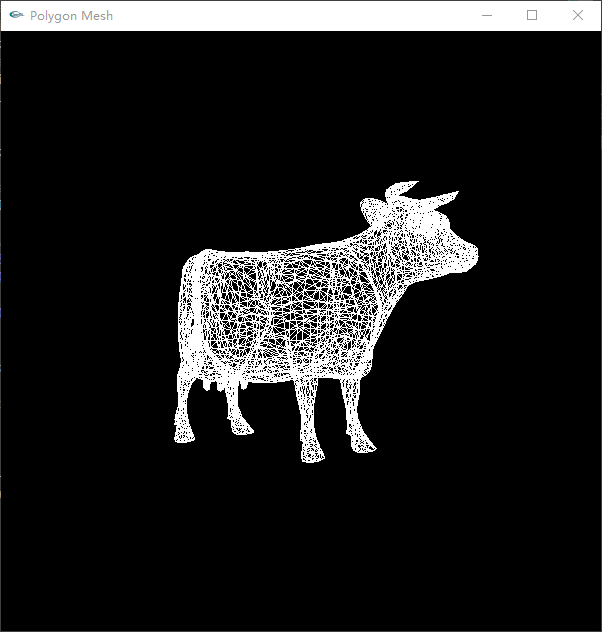
\includegraphics[width=0.33\linewidth]{fig/cow1.png} &
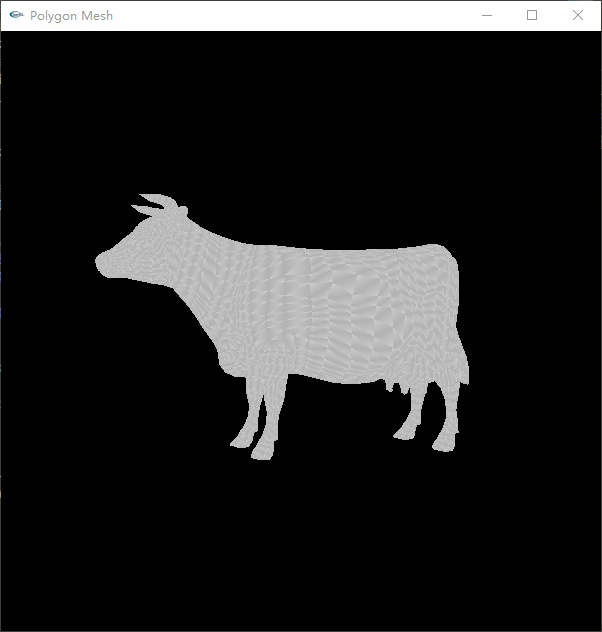
\includegraphics[width=0.33\linewidth]{fig/cow2.png} &

\includegraphics[width=0.33\linewidth]{fig/cow3.png}
\end{tabular}
\caption{cow.obj模型}
\label{fig:cow}
\end{figure}

\begin{figure}[H]
\centering
\begin{tabular}{ccc}
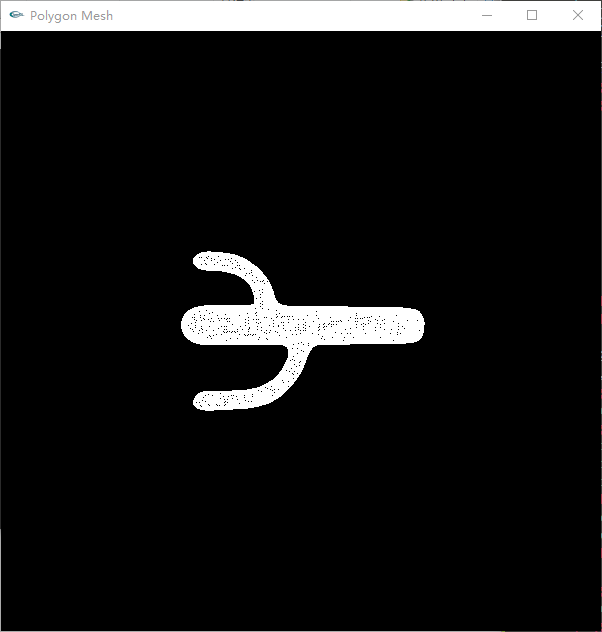
\includegraphics[width=0.33\linewidth]{fig/cactus1.png} &
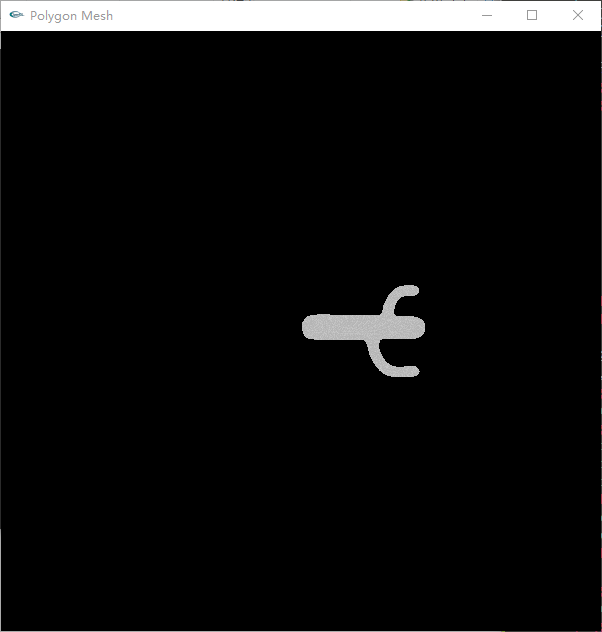
\includegraphics[width=0.33\linewidth]{fig/cactus2.png} &
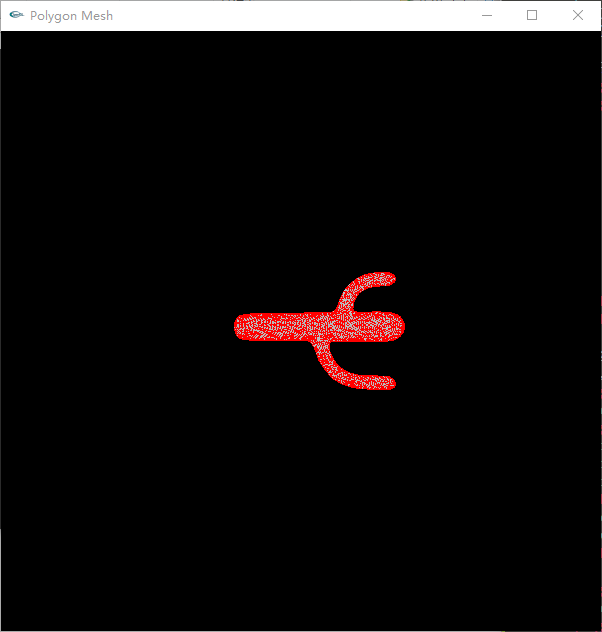
\includegraphics[width=0.33\linewidth]{fig/cactus3.png}
\end{tabular}
\caption{cactus.ply模型}
\label{fig:cactus}
\end{figure}

\begin{figure}[H]
\centering
\begin{tabular}{ccc}
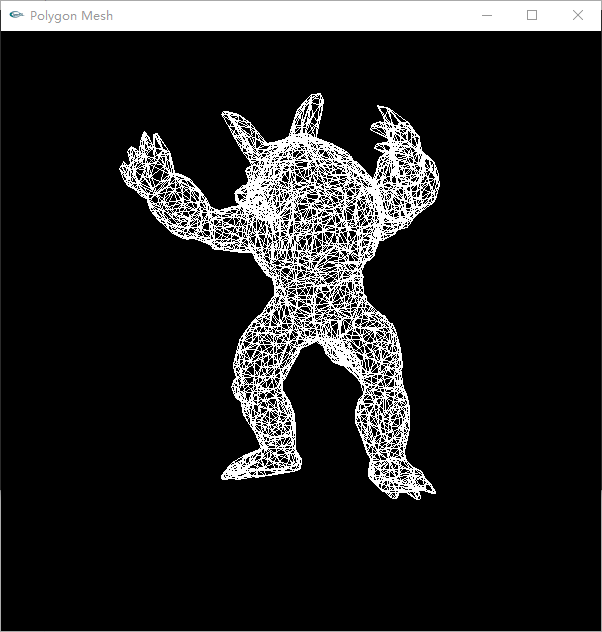
\includegraphics[width=0.33\linewidth]{fig/armadillo1.png} &
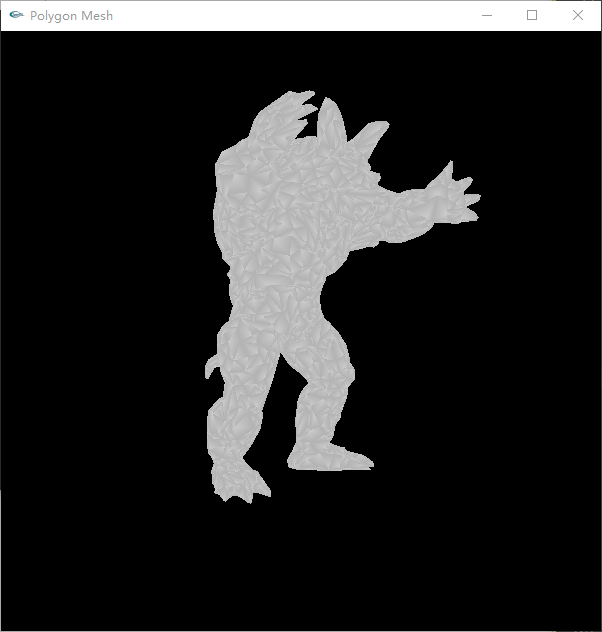
\includegraphics[width=0.33\linewidth]{fig/armadillo2.png} &
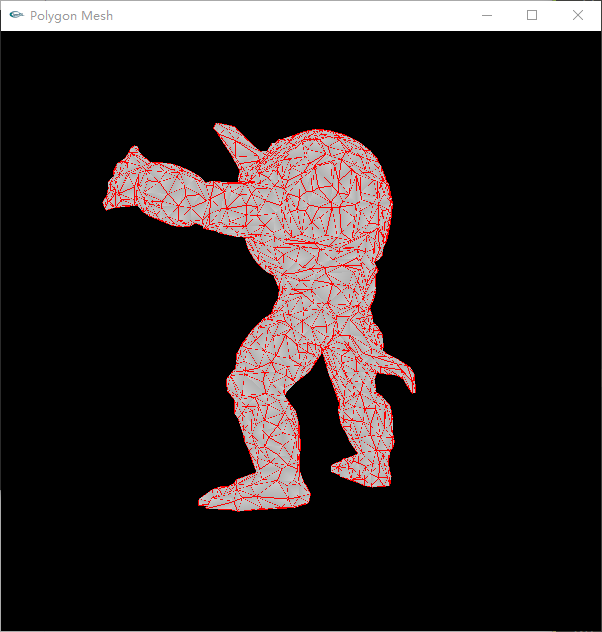
\includegraphics[width=0.33\linewidth]{fig/armadillo3.png}
\end{tabular}
\caption{armadillo.off模型}
\label{fig:armadillo}
\end{figure}

\appendixconfig
\appendix
\section{源代码}

\verb'mesh.h'包含三种格式文件的读取器。
\lstinputlisting{mesh.h}

\verb'mesh.cpp'核心显示代码。
\lstinputlisting{mesh.cpp}

编译指令如下:
\begin{flushleft}
\verb'g++ mesh.cpp -DOBJ=1 -I.\include -L.\lib -lglu32 -lglut32 -lopengl32 -o cow.exe'\\
\verb'g++ mesh.cpp -DPLY=1 -I.\include -L.\lib -lglu32 -lglut32 -lopengl32 -o cactus.exe'\\
\verb'g++ mesh.cpp -DOFF=1 -I.\include -L.\lib -lglu32 -lglut32 -lopengl32 -o armadillo.exe'
\end{flushleft}

\end{document}
% 题目:用 OpenGL 实现简单的多边形网格数据读取和操作。
% 功能要求:
% 1. 支持读取.obj、 .off 和.ply 格式的多边形网格文件,见附带的数据文件;
% 2. 对载入的多边形网格进行平移和旋转操作;
% 3. 实现多边形网格的 Wireframe、 Flat 和 Flat lines 显示效果,如图 2 所示。
% 4. 语言不限,开发平台不限,具体效果展示允许略有差异。
% 实现提示:
% 1. 功能可参考 MeshLab 项目(http://meshlab.sourceforge.net/)
% 2. 允许使用轻量级的第三方支持库,但请留意提交的作业因缺失库文件而不能运行。

% 要求:
% 1. 作业按百分制评分, 没交作业算 0 分;
% 2. 提交代码文件,缺源代码文件的作业成绩减 10 分;
% 3. 提交直接可执行的程序文件或脚本文件,不能运行的程序(含出错,缺 dll 文件等) 作业成绩减 10 分;
% 4. 作业文档,包含简要的程序文件说明,运行方法,以及程序运行结果截图,缺文档的作业成绩减 10 分;
% 5. 发现作业抄袭的本次作业算 0 分。
% 说明:
% 两个题目均需完成,可分开两个 Demo。
% 以小组为单位,组长收齐小组内各位同学的作业,作业用 zip 格式文件打包提交(请尽量减少压缩包文件的体积),以附件方式发送到课程邮箱。
% 请于 11 月 24 日 24:00 前提交。
% 邮件名和压缩包文件名格式如下:班级 + 学号 + 姓名 + HW5
% 例: 16 计科+16000001+张三+HW5